% !TeX program = lualatex
% !TeX encoding = utf8
% !TeX spellcheck = uk_UA
% !BIB program = biber

\documentclass[10pt]{beamer}
\usetheme{QuantumChemistry}
\usepackage{QuantumChemistry}
%============================================================================
\title[Лекції з квантової хімії]{\huge\bfseries Атом гелію \\\ce{He}}
\subtitle{Лекції з квантової хімії}
\date{}
\author{Пономаренко С. М.}
%============================================================================
\addbibresource{../Bibliography/QuantumChemistry.bib}
\AtEveryCitekey{\clearfield{url}\clearfield{doi}}

\graphicspath{{pictures/}}

\newcommand{\xdownarrow}[1]{%
  {\left\downarrow\vbox to #1{}\right.\kern-\nulldelimiterspace}
}
\newcommand{\xuparrow}[1]{%
  {\left\uparrow\vbox to #1{}\right.\kern-\nulldelimiterspace}
}





\begin{document}

%============================================================================
\begin{frame}
	\thispagestyle{empty}
	\titlepage
\end{frame}






%============================================================================
\section{Загальні відомості}
%============================================================================





\begin{frame}{}{}
	%----------------------------------------------------------------------------
	\begin{center}
		\hspace*{2.5ex}\includegraphics[width=0.6\linewidth]{HeSpectra}  \\

		H\hspace*{1.0ex} \includegraphics[width=0.6\linewidth]{Hydrogen}    \\

		He \includegraphics[width=0.6\linewidth]{Helium}
	\end{center}
	\href{https://www.nist.gov/pml/atomic-spectra-database}{Atomic Spectra Database}
	%----------------------------------------------------------------------------
\end{frame}
%============================================================================





%============================================================================
\begin{frame}{Енергетичні рівні атома He}{}
	%----------------------------------------------------------------------------
	\begin{columns}
		\begin{column}{0.6\linewidth}
			\begin{center}
				\includegraphics[width=1\linewidth]{SpectraHe}
			\end{center}
		\end{column}
		\begin{column}{0.4\linewidth}\small
			В спектрі газоподібного гелію є трикратно вироджені рівні~--- \emph{\color{blue}триплет}, та невироджені~--- \emph{\color{red}синглет}. Атоми, які утворюють спектроскопічний триплет називаються \emph{\color{blue}ортогелієм}, а синглет~--- \emph{\color{red}парагелієм}.
			Між цими станами \emph{майже} неможливі квантові переходи.
		\end{column}
	\end{columns}
	\medskip
	\begin{block}{}\scriptsize\justifying
		\alert{Інтеркомбінацційні квантові переходи} в атомних системах --- квантові переходи між станами системи, що супроводжуються зміною її повного спіну, тобто переходи між рівнями енергії з різною мультиплетністю. Відбуваються, наприклад, за рахунок спін-орбітальної (тобто, магнітної) взаємодії. Як правило, такі переходи відбуваються без випромінювання.
	\end{block}
	%----------------------------------------------------------------------------
\end{frame}
%============================================================================





%============================================================================
\begin{frame}{Стаціонарне рівняння Шредінґера атома \ce{He}}{}
	%----------------------------------------------------------------------------
	\begin{equation*}
		\tcbhighmath{\hat{H}\Psi(\vxi_1, \vxi_2) = E\Psi(\vxi_1, \vxi_2).}
	\end{equation*}
	\begin{columns}[T]
		\column{.7\textwidth} % column designated by a command
		\begin{equation*}
			\hat{H} = \left( -\frac12 \vec{\nabla}^2_1  - \frac{Z}{r_1} \right) + \left( - \frac12 \vec{\nabla}^2_2 - \frac{Z}{r_2} \right)  + \frac{1}{r_{12}}.
		\end{equation*}

		%    \begin{enumerate}\footnotesize
		%        \item Гамільтоніан системи електрично взаємодіючих частинок (без магнітного поля) не містить операторів спіну --- не впливає на спінові змінні.
		%        \item Однак, існує своєрідна залежність енергії системи від її повного спіну.
		%    \end{enumerate}

		\[
			\Psi = \Psi (\vxi_1, \vxi_2)
		\]
		\[
			\vxi_1 = (\vec{r}_1, \sigma_1), \quad 	\vxi_2 = (\vec{r}_2, \sigma_2).
		\]

		$\vec{r}_1 = (x_1, y_1, z_1)$ та  $\vec{r}_2 = (x_2, y_2, z_2)$ --- просторові координати електрона,

		$\sigma_1$ та $\sigma_2$ --- спінові координати.

		\
		\column{.3\textwidth}
		\begin{center}
			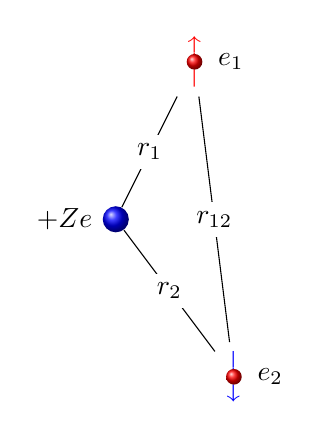
\begin{tikzpicture}[]
				\node[circle, ball color = blue] (Z) at (0,0) {}; \node[left=5pt] at (Z) {$+Ze$};
				\node[red, font=\large] (e1) at (1,2) {$\xuparrow{10pt}$};
				\node[blue] (e2)  at (1.5,-2){$\xdownarrow{10pt}$};
				\node[circle, ball color = red, inner sep= 2pt] at (e1)   {}; \node[right=5pt] at (e1) {$e_1$};
				\node[circle, ball color = red, inner sep= 2pt] at (e2)  {}; \node[right=5pt] at (e2) {$e_2$};

				\draw (Z) -- node[fill=white] {$r_1$} (e1) (Z) -- node[fill=white] {$r_2$ }(e2) (e1) -- node[fill=white] {$r_{12}$}(e2);
			\end{tikzpicture}
		\end{center}
	\end{columns}
	%----------------------------------------------------------------------------
\end{frame}
%============================================================================



\begin{frame}{Хімічна точність}


\begin{block}{}
    У квантовій хімії термін \textbf{«хімічна точність»} (\textit{chemical accuracy}) означає здатність методу відтворювати енергії молекулярних систем із похибкою не більше ніж приблизно
\[
1 \ \text{kcal/mol} \approx 4.184 \ \text{kJ/mol} \approx 0.043 \ \text{eV} \approx 1.6 \times 10^{-3} \ \text{a.u. (Hartree)}.
\]
\end{block}

\begin{itemize}
  \item Це порядок величини характерних енергій хімічних процесів: водневих зв’язків, ізомеризацій, активаційних бар’єрів.
  \item Різниця навіть у $\sim 1$ ккал/моль може суттєво змінити передбачення рівноваги або константи швидкості реакції.
  \item Якщо метод відтворює енергії з такою точністю, його можна вважати придатним для \textbf{надійного моделювання хімічних властивостей}.
\end{itemize}


\begin{alertblock}{}\justifying
  У контексті квантових обчислень саме «chemical accuracy» вважається \textit{«священним Граалем»}: досягнення цієї точності для реальних молекул означає прорив.
\end{alertblock}

\end{frame}




%============================================================================
\begin{frame}{Теорія збурень}{}
	%---------------------------------------------------------------------------
	Основна ідея теорії збурень --- всі взаємодії в системі можна умовно розділити на <<основні>> і <<збурення>>, --- гамільтоніан системи можна представити у вигляді:
	\begin{equation*}
		\hat{H} = \hat{H}^0 + \hat{V},
	\end{equation*}
	де  $\hat{H}^0$~--- <<незбурений>> гамільтоніан:
	\begin{equation*}
		\hat{H}^0\psi_n^{(0)} = E_n\psi_n^{(0)}.
	\end{equation*}
	Функції $\{\psi_n^{(0)}\}$ --- орбіталі.% --- метод збурень природнім способом реалізує одноелектронне наближення.

	Доданок $\hat{V}$ в припущенні <<малості>> --- <<збурення>>.

	Перше наближення теорії збурень:
	\begin{equation*}\label{PerturbedValues}
		E_n = E_n^{(0)} + \bracket<\psi_n^{(0)}|\hat{V}|\psi_n^{(0)}>, \quad
		\psi_n = \psi_n^{(0)} + \sum\limits_{\substack{m\\m \neq n}} \frac{\bracket<\psi_n^{(0)}|\hat{V}|\psi_m^{(0)}>}{E_n^{(0)} - E_m^{(0)}} \psi_m^{(0)}.
	\end{equation*}
	%---------------------------------------------------------------------------
\end{frame}





%============================================================================
\section{Теорія збурень}
%============================================================================





\begin{frame}{Теорія збурень}{Атом гелію}
	%----------------------------------------------------------------------------
	\begin{gather*}
		\hat H =
		\underbrace{\left( -\frac{\hbar}{2m_e}\vec{\nabla}^2_1 - \frac{Ze^2}{r_1} \right)}_{\hat h_1} + \\
		+
		\underbrace{\left( -\frac{\hbar}{2m_e}\vec{\nabla}^2_2 - \frac{Ze^2}{r_2} \right)}_{\hat h_2} +
		\underbrace{\frac{e^2}{r_{12}}}_{\hat V_{12}} = \\
		= \underbrace{\hat h_1 + \hat h_2}_\text{Незбурений гамільтоніан}
		+
		\underbrace{\hat V_{12}}_\text{збурення?}  = \\
		= \hat H^{0} + \hat V_{12}
	\end{gather*}
	Для основної задачі з гамільтоніаном:
	\begin{equation*}
		\hat{H}^0 = \hat{h}_1 + \hat{h}_2.
	\end{equation*}
	%----------------------------------------------------------------------------
\end{frame}
%============================================================================





%============================================================================
\begin{frame}{Теорія збурень}{Парагелій}
	%----------------------------------------------------------------------------
	\only<1>{
		Для парагелію $\gamma = \alpha(1)\beta(2) - \alpha(2)\beta(1)$%
		\tikz[scale=0.25, baseline = (base),
			upspinarrow/.pic = {\draw[-latex, red] (0,-0.5) -- (0, 0.5);},
			downspinarrow/.pic = {\draw[latex-,blue] (0,-0.5) -- (0, 0.5);}
		]{
			\def\distance{1.5}
			\draw[ultra thick]  (0,0) -- pic[pos=0.3] {upspinarrow}  pic[pos=0.7] {downspinarrow}+(2,0)  node[right] {$n_{1,2} = (1s)$};
			\path (-1.5, -1) rectangle (1.5,2.5);
			\coordinate (base) at (0, -0.5);
		}:
		\begin{equation*}
			\Psi_0(\vec{r}_1, \vec{r}_2) = (1s)_1(1s)_2, \quad (1s) = \frac{Z^{3/2}}{\sqrt{4\pi}} e^{-Zr} .
		\end{equation*}

		Енергія незбуреного основного стану являє собою суму енергій двох воднеподібних атомів:
		\begin{equation*}
			E^{0} = -Z^2.
		\end{equation*}

		Перша поправка до енергії в теорії збурень:
		\begin{equation*}
			E^{(1)} = \bracket<{\Psi_0}|{\hat{V}}|{\Psi_0}> \equiv J = \frac{Z^6}{\pi^2} \int\limits_{V_1}\int\limits_{V_2}\frac{1}{r_{12}} e^{-2Z(r_1 + r_2)} dV_1dV_2 = + \frac58 Z.
		\end{equation*}
		$J$~--- кулонівський інтеграл.
		Енергія атома \ce{He} :
		\begin{equation*}\label{E_He_perturb}
			E = E^{(0)} + J =  -Z^2 + \frac58 Z.
		\end{equation*}
	}
	\only<2>{
		Розраховане значення $Z = 2$, $\Rightarrow$ $E = - 4 + \frac54 = -2.75$~Ха.

		\medskip

		Експериментальне значення $-2.9037$~Ха.

		%       Теорема віріалу  $\left\langle T \right\rangle  = - E $
		%
		%		Порушення в теорії збурень:
		%
		%		повна енергія  $\Rightarrow$ $\ E  = -Z^2 +\frac58 Z$,
		%
		%		кінетична  $\Rightarrow$ $\left\langle T \right\rangle   = Z^2$,
		%
		%		$Z^2 \neq Z^2 -\frac{5}{16} Z$.

		\begin{center}
			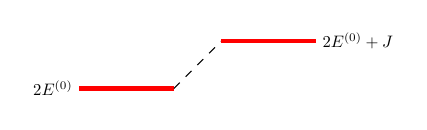
\begin{tikzpicture}[scale=0.6, every node/.style={scale=0.6}]
				\draw[ultra thick, red] (0,0) node[left, black] {$2E^{(0)}$} -- (2,0);
				\draw[dashed](2,0) -- (3,1);
				\draw[ultra thick, red] (3,1) -- (5,1) node[black, right] {$2E^{(0)} + J$};
			\end{tikzpicture}
		\end{center}
	}
	%----------------------------------------------------------------------------
\end{frame}
%============================================================================





%============================================================================
%\begin{frame}{Теорія збурень}{Ортогелій}
%	%----------------------------------------------------------------------------
%	\only<1>{
%		Для ортогелію $\gamma = \alpha(1) \alpha(2)$
%		\tikz[scale=0.25, baseline = (base),
%			upspinarrow/.pic = {\draw[-latex, red] (0,-0.5) -- (0, 0.5);},
%			downspinarrow/.pic = {\draw[latex-,blue] (0,-0.5) -- (0, 0.5);}
%		]{
%			\def\distance{2.5}
%			\draw[ultra thick]  (0,0) -- pic[pos=0.3] {upspinarrow}  +(2, 0) node[right] {$n_1 = (1s)$};
%			\draw[ultra thick]  (0,\distance) -- pic[pos=0.7] {upspinarrow} +(2,0) node[right] {$n_2 = (2s)$};
%			\path (-1.5, -1) rectangle (1.5,2.5);
%			\coordinate (base) at (0, 1);
%		}:
%		\begin{equation*}
%			\Psi_0(\vec{r}_1, \vec{r}_2) = \frac1{\sqrt{2}}[(1s)_1(2s)_2 -(2s)_1(1s)_2],
%		\end{equation*}
%		\[
%			\quad (1s) = \frac{Z^{3/2}}{\sqrt{4\pi}} e^{-Zr}, (2s) = \frac{Z^{3/2}}{4\sqrt{2\pi}} (2 - Zr)e^{-\frac{Z}{2}r}
%		\]
%		Перша поправка до енергії в теорії збурень:
%		\begin{multline*}
%			E^{(1)} = \bracket<\Psi_0|\hat{V}|\Psi_0> = \\ = \bracket<(1s)_1(2s)_2|\hat{V}|(1s)_1(2s)_2> - \bracket<(1s)_1(2s)_2|\hat{V}|(2s)_1(1s)_2> = J - K.
%		\end{multline*}
%		$J$~--- кулонівський інтеграл, $K$~--- обмінний інтеграл.
%		\[
%			J = \pgfmathparse{11.41569905002/27.2113845}\pgfmathresult, \quad K =  \pgfmathparse{1.193796374161/27.2113845}\pgfmathresult
%		\]
%	}
%	\only<2>{
%	Для ортогелію $E = - 2 - \frac12 + J - K \approx \pgfmathparse{-2-0.5 + 11.41569905002/27.2113845 - 1.193796374161/27.2113845}\pgfmathresult$~Ха.
%
%	Експериментальне значення $-2.18$~Ха.
%
%	{\scriptsize \fullcite{VoicuDolocan}}
%
%	\begin{center}
%		\begin{tikzpicture}[scale=0.6, every node/.style={scale=0.6}]
%			\draw[ultra thick, red] (0,2) node[left, black] {$E_1 + E_2$} -- (2,2);
%			\draw[dashed](2,2) -- (3,3);
%			\draw[ultra thick, red] (3,3) -- (5,3) node[right, black] {$E_1 + E_2 + J - K$};
%		\end{tikzpicture}
%	\end{center}
%	}
%\end{frame}





%============================================================================
\section{Варіаційний метод}
%============================================================================





\begin{frame}{Варіаційний метод}{}
	%----------------------------------------------------------------------------
	\only<1>{%
		Енергію системи в стані $\Psi$ можна розрахувати як:
		\begin{equation*}
			E[\Psi]  = \bracket<{\Psi}|{\hat{H}}|{\Psi}> = \int \Psi^* \hat{H} \Psi d\xi, \quad \int \Psi^*  \Psi d\xi = 1.
		\end{equation*}
		Застосуємо варіаційний принцип $\delta E = 0$
		\[
			\delta E =  \int \delta \Psi^* \hat{H} \Psi d\xi + \int \Psi^* \hat{H} \delta \Psi d\xi = 0
		\]
		Варіація умови нормування
		\[
			\delta \left(-\lambda \int \Psi^*  \Psi d\xi - 1\right)=  -\lambda \int \delta \Psi^* \Psi d\xi -\lambda  \int  \Psi^*  \delta \Psi d\xi = 0
		\]
		\[
			\int \delta \Psi^* \left( \hat{H} - \lambda\right) \Psi d\xi + \int \delta \Psi \left( \hat{H} - \lambda\right)^{\dagger} \Psi^* d\xi = 0  \rightarrow \hat{H}  \Psi = \lambda  \Psi, \lambda = E
		\]
		Якщо ми знаємо точну функцію $\Psi$ $\rightarrow$ отримуємо рівняння Шредінґера.
		\begin{center}
			\alert{Зазвичай ми не знаємо точну функцію!}
		\end{center}
	}
	\only<2>{%
		Припустимо, що довільна функція $\tilde{\Psi} = \sum\limits_m C_m\Psi_m$ є розв'язком, $(\sum\limits_m|C_m|^2 = 1)$, $\bracket<\tilde{\Psi}|\tilde{\Psi}> = 1$, розкладена в ряд по точним (але невідомим) власним функціям гамільтоніана $\hat H$ :

		\begin{equation*}
			E[\Psi]  = \bracket<{\tilde\Psi}|{\hat{H}}|{\tilde\Psi}> = \sum\limits_m |C_m|^2 E_m.
		\end{equation*}

		Нехай $E_0$ найменше  значення енергії основного стану гамільтоніана $\hat{H}$, тоді
		\begin{equation*}
			E[\tilde\Psi]  = \bracket<{\tilde\Psi}|{\hat{H}}|{\tilde\Psi}> = \sum\limits_m |C_m|^2 E_m \ge \sum\limits_m |C_m|^2 E_0  = E_0.
		\end{equation*}
		\begin{alertblock}{}\centering
			Енергія обчислена з довільною функцією $\tilde\Psi$  буде оцінкою зверху для точного значення енергії основного стану
		\end{alertblock}
	}
	\only<3>%
	{    \framesubtitle<3>{Реалізація методу}
		Варіаційний метод полягає в тому, щоб використати для розв'язку якусь пробну функцію змінних системи  $\Psi (\lambda_i)$, що залежить від декількох параметрів $\lambda_i$, яка задовільняє умові нормування, тоді:
		\[
			E[\tilde\Psi]  = E[\tilde\Psi(\lambda_1, \lambda_2, \ldots)],
		\]
		умова мінімуму дає $\delta E[\Psi] = 0$:
		\[
			\frac{\partial E}{\partial \lambda_1} = 0, \quad \frac{\partial E}{\partial \lambda_2} = 0, \ldots.
		\]
		Система цих рівнянь визначає параметри $\lambda_{i_{\min}}$, для яких
		\[
			E_{\min}[\tilde\Psi(\lambda_{1_{\min}}, \lambda_{2_{\min}}, \ldots)] \ge E_0.
		\]
	}
	%----------------------------------------------------------------------------
\end{frame}
%============================================================================





%============================================================================
\begin{frame}{Варіаційний метод}{Атом гелію}
	%----------------------------------------------------------------------------
	<<Пробні>> орбіталі --- 1s-функції воднеподібного атому:
	\begin{equation*}\label{coordinate_ground_state_parahelium}
		\Psi_0(\vec{r}_1, \vec{r}_2) = (1s)_1(1s)_2 = \frac{\zeta^{3}}{\pi}e^{-\zeta(r_1 + r_2)}.
	\end{equation*}
	Заряд ядра $\zeta$ --- параметр, який варіюється --- грунтується на інтуїтивно зрозумілій ідеї \alert{екранування} електронами заряду ядра. {\scriptsize Один із електронів екранує заряд ядра, в результаті чого інший електрон <<відчуває>> не величину $Z$, а вже дещо менше її значення $\zeta$. Для ефективності екранування вводять величину}
	\begin{equation*}
		\sigma = Z - \zeta,
	\end{equation*}

	яка називається \alert{константою екранування}.
	%----------------------------------------------------------------------------
\end{frame}
%============================================================================





%============================================================================
\begin{frame}{Варіаційний метод}{Атом гелію}
	Для розв'язання цієї задачі перепишемо гамільтоніан  у більш зручному для інтегрування вигляді:
	\begin{equation*}\label{}
		\hat{H} = \left[ -\frac12 \vec{\nabla}^2_1  -\frac12 \vec{\nabla}^2_2 - \frac{\zeta}{r_2} - \frac{\zeta}{r_1} \right] + \left[- \frac{Z-\zeta}{r_2} - \frac{Z-\zeta}{r_1} + \frac{1}{r_{12}} \right].
	\end{equation*}

	Функціонал енергії матиме вигляд:
	\begin{equation*}
		E = -\zeta^2 - 2(Z - \zeta)\zeta + \frac58 \zeta = \zeta^2 + \zeta\left( \frac58 - 2Z\right) .
	\end{equation*}
	Із умови $\dfrac{\partial E}{\partial \zeta} = 0$ знаходимо $	\zeta_{\min} = Z - \frac{5}{16}$.
	Підставимо значення $\zeta_{\min}$ в функціонал енергії  і отримаємо значення енергії основного стану атома гелію:
	\begin{equation*}\label{}
		E = -\left( Z - 5/16\right)^2 = -\zeta^2 = -2.85 \text{~Ха}.
	\end{equation*}
	%----------------------------------------------------------------------------
\end{frame}
%============================================================================





%============================================================================
\begin{frame}{Варіаційний метод}{Теорема віріалу}\small
	%----------------------------------------------------------------------------
	Хвильова функція покращена за допомогою варіаційного методу дає не лише кращий результат для енергії основного стану гелію, але і задовольняє теоремі віріалу. Так, середнє значення кінетичної енергії електронів:
	\[
		\left\langle T \right\rangle = \zeta^2 = - E,
	\]
	\begin{itemize}
		\item  Кулонівська взаємодія між електронами зводиться не лише до відштовхування між електронами, а і до ефекту екранування, що відбивається в $\zeta$.
		\item Екранування набагато сильніше позначається саме на кінетичній енергії електронів, оскільки саме вона залежить квадратично від ефективного заряду ядра $\zeta$, тоді як середня потенціальна енергія міжелектронної взаємодії  $\left\langle V_{ee} \right\rangle = \frac58 \zeta$ залежить від нього лише лінійно.
	\end{itemize}
	%----------------------------------------------------------------------------
\end{frame}
%============================================================================





%============================================================================
\begin{frame}[t]{Екранування}\small
	%----------------------------------------------------------------------------
	\begin{columns}
		\begin{column}{0.4\linewidth}
			\begin{center}
				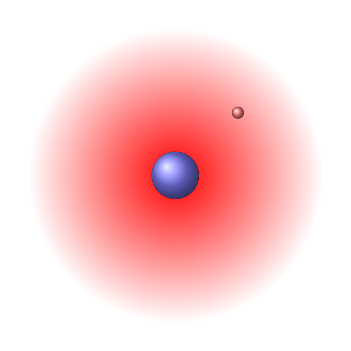
\begin{tikzpicture}[scale=0.75]
					\path[inner color=red, outer color=white] (0,0) circle(2.5);
					\fill[ball color=blue!50] (0,0) circle (0.4);
					\fill[ball color=red!50]  (45:1.5) coordinate (E2) circle (0.1);
				\end{tikzpicture}
			\end{center}
		\end{column}
		\begin{column}{0.6\linewidth}\centering
			Ефективний заряд

			\[\tcbhighmath[drop fuzzy shadow]{\zeta_{\min} =  Z - 5/16 = 1.6875}\]

			Стала екранування

			\[\tcbhighmath[drop fuzzy shadow]{\sigma = Z - \zeta_{\min} = 5/16 = 0.3125}\]
		\end{column}
	\end{columns}
	\bigskip

	\begin{block}{}
		Кожен з електронів частково «екранує» інший електрон від ядра, в результаті чого електрони притягуються до ядра слабше; це виражається в уявному зменшенні заряду ядра гелію, який дорівнює не $2$, а $\approx 1.7$.
	\end{block}
	%----------------------------------------------------------------------------
\end{frame}





%============================================================================
\section{Методи самоузгодженого поля}
%============================================================================





\begin{frame}{Метод самоузгодженого поля}{Метод Хартрі (1927)}
	%----------------------------------------------------------------------------
	\begin{columns}
		\begin{column}{0.4\linewidth}
			\begin{center}
				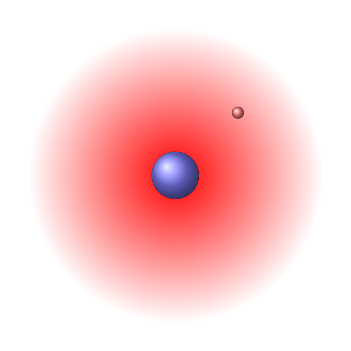
\begin{tikzpicture}[scale=0.75]
					\path[inner color=red, outer color=white] (0,0) circle(2.5);
					\fill[ball color=blue!50] (0,0) circle (0.4);
					\fill[ball color=red!50]  (45:1.5) coordinate (E2) circle (0.1);
				\end{tikzpicture}
			\end{center}
		\end{column}
		\begin{column}{0.6\linewidth}
			Ідея методу самоузгодженого поля полягає в тому, що взаємодія електрона з іншим електроном замінюється його взаємодією із усередненим полем, створюваним ядром та іншим електроном.
		\end{column}
	\end{columns}

	\begin{overprint}
		\onslide<1>
		Для реалізації метода необхідні припущення:
		\begin{itemize}\small
			\item Кожен електрон характеризується своєю хвильовою функцією: $\psi_1$ та $\psi_2$, відповідно, які нормовані $\int |\psi_1|^2 dV_1 = 1$,  $\int |\psi_2|^2 dV_2 = 1$;
			\item Хвильова функція системи електронів задається у вигляді: $\Psi = \psi_1 \psi_2$;
			\item Рівняння методу виводяться на основі варіаційного принципу.
		\end{itemize}
		\onslide<2>
		Рівняння Хартрі (в атомній системі одиниць):
		\begin{align*}
			\left(-\frac12 \nabla_1^2  - \frac{1}{r_1} \right)\psi_1 + \int\frac{|\psi_2|^2}{r_{12}} dV_2 \cdot \psi_1 & = \varepsilon_1 \psi_1, \\
			\left(-\frac12 \nabla_2^2  - \frac{1}{r_2}\right)\psi_2 + \int\frac{|\psi_1|^2}{r_{12}} dV_1 \cdot \psi_2  & = \varepsilon_2 \psi_2.
		\end{align*}
		\onslide<3>
		Енергія атома методом Хартрі $E = \bracket<{\Psi}|{\hat{H}}|{\Psi}>$:
		\begin{multline*}
			E =  \int \psi^*_1 \left( -\frac12 \nabla_1^2 - \frac{1}{r_{1}}\right) \psi_1 dV_1 + \int \psi^*_2 \left( -\frac12 \nabla_2и и ^2 - \frac{1}{r_{2}}\right) \psi_2 dV_2 + \\ +  \int\frac{|\psi_1|^2 |\psi_2|^2}{r_{12}} dV_1 dV_2
			= \varepsilon_1 + \varepsilon_2 - \int\frac{|\psi_1|^2 |\psi_2|^2}{r_{12}} dV_1 dV_2.
		\end{multline*}
	\end{overprint}
	%----------------------------------------------------------------------------
\end{frame}
%============================================================================





%============================================================================
\begin{frame}{Метод Хартрі}{Процедура розв'язку рівнянь Хaртрі}
	%----------------------------------------------------------------------------
	\begin{columns}[T]
		\begin{column}{0.35\linewidth}
			\begin{tikzpicture}[
					every node/.style={font=\scriptsize, very thin, scale=.7},
					node distance=1.2cm,
					startstop/.style={rectangle, rounded corners, minimum width=1cm, minimum height=0.5cm,text centered, draw=black, fill=red!30},
					process/.style={rectangle, minimum width=1cm, minimum height=0.5cm, text centered, draw=black, fill=orange!30},
					io/.style={trapezium, trapezium left angle=70, trapezium right angle=110, minimum width=1cm, minimum height=0.5cm, text centered, draw=black, fill=blue!30},
					decision/.style={diamond, minimum width=1cm, minimum height=0.5cm, text centered, draw=black, fill=green!30},
				]

				\node (node0) [io] {$\{\psi_1^{(0)}, \psi_2^{(0)}\}$};
				\node (node1) [process, below of=node0]  {$\int \frac{|\psi_1^{(k)}|^2}{r_{12}} dV_1$, $\int \frac{|\psi_2^{(k)}|^2}{r_{12}} dV_2$};
				\node (node2) [process, below of=node1]               {Розв'язок рівняннь Хартрі};
				\node (node3) [io, below=0.5cm of node2]               {$\{\psi_1^{(k)}, \psi_2^{(k)}\}$};
				\node (node4) [decision, below=0.5cm of node3]               {$\left| E^{(k)} - E^{(k - 1)}\right| \le \delta$};
				\node (node5) [startstop, below=0.5cm of node4]               {Розрахунок енергії, властивостей...};


				\draw[-latex] (node0) -- (node1);
				\draw[-latex] (node1) -- (node2);
				\draw[-latex] (node2) -- (node3);
				\draw[-latex] (node3) -- (node4);
				\draw[-latex] (node4.west) -- node[above] {Ні} +(-1,0) coordinate (N) -- node[rotate=90, above] {Продовження ітерацій} (node1.west-|N) -- (node1.west);
				\draw[-latex] (node4.east) -- node[above] {Так} +(1,0) coordinate (Y) -- node[rotate=-90, below] {Вихід}  (node5.west-|Y) -- (node5.east);
			\end{tikzpicture}
		\end{column}
		\begin{column}{0.55\linewidth}\footnotesize
			\alert{Ітераційна} процедура була названа самоузгодженням, а тому метод Хартрі отримав назву методу самоузгодженого поля (SCF).
			\begin{itemize}
				\item  На першому етапі необхідно задати набір деяких початкових функцій $\{\psi_1^{(0)}, \psi_2^{(0)}\}$ в \alert{чисельному вигляді}. Можна вибрати функції можна обрати атомні орбіталі воднеподібного атома.
				\item Чим точніше вибрано початкові функції, тим менше буде ітерацій. Для зменшення циклів (можна взяти атомні воднеподібні орбіталі з урахуванням екранування).
				\item Розрахунки цим методом дають лише чисельні результати.
			\end{itemize}

		\end{column}
	\end{columns}
	%----------------------------------------------------------------------------
\end{frame}
%============================================================================





%============================================================================
\begin{frame}{Недоліки методу Хартрі}{}
	%----------------------------------------------------------------------------
	Оскільки, для отримання $\Psi$-функції системи необхідно перемножити орбіталі, а тому:
	\begin{itemize}
		\item не враховується принцип Паулі для електронів;

		      {\footnotesize Існує ненульова ймовірність знаходження електронів в одні і тій же точці простору, що неможливо для електронів з паралельними спінами. Для електронів з антипаралельними спінами все добре.}
		\item не враховується кореляція в русі електронів завдяки кулонівському відштовхуванню.

		      {\footnotesize  Існує ненульова ймовірність знаходження електронів в одні і тій же точці простору, що неможливо завдяки їх кулонівському відштовхуванню. Не є добре для електронів з будь-якою орієнтацією спінів.}
	\end{itemize}
	%----------------------------------------------------------------------------
\end{frame}
%============================================================================





%============================================================================
\begin{frame}{Метод самоузгодженого поля}{Метод Хартрі-Фока}
	%----------------------------------------------------------------------------
	Для врахування принципу Паулі, В. Фок запропонував представити хвильову функцію у вигляді детермінанту Слейтера:
	\begin{equation*}
		\Psi (\vxi_1, \vxi_2)={\frac {1}{\sqrt {2}}}
		\left|
		{
		\begin{matrix}
			\psi_{1}(\vxi_1) & \psi_{2}(\vxi_1) \\
			\psi_{1}(\vxi_2) & \psi_{2}(\vxi_2)
		\end{matrix}
		}
		\right|.
	\end{equation*}

	\begin{overprint}
		\onslide<1>
		Для реалізації метода необхідні припущення:
		\begin{itemize}
			\item Кожен електрон характеризується своєю хвильовою функцією: $\psi_1$ та $\psi_2$, відповідно, які нормовані $\int |\psi_1|^2 dV_1 = 1$,  $\int |\psi_2|^2 dV_2 = 1$;
			\item Рівняння методу виводяться на основі варіаційного принципу.
		\end{itemize}
		\onslide<2>
		Канонічні рівняння Хартрі-Фока (в атомній системі одиниць):
		{\footnotesize
		\begin{align*}
			\hat{h}_1\psi_1(\vxi_1) +
			\int\frac{|\psi_2(\vxi_2)|^2}{r_{12}} d(2) \cdot \psi_1 (\vxi_1) -
			\int \frac{\psi_2(\vxi_2)\psi_1(\vxi_2)}{r_{12}}d(2)\cdot\psi_1(\vxi_1) \\
			 & = \varepsilon_1 \psi_1(\vxi_1),                                        \\
			% ----------------
			\hat{h}_2\psi_2(\vxi_2) +
			\int\frac{|\psi_1(\vxi_1)|^2}{r_{12}} d(1) \cdot \psi_2 (\vxi_2) -
			\int \frac{\psi_1(\vxi_1)\psi_2(\vxi_1)}{r_{12}}d(1)\cdot\psi_2(\vxi_2) \\
			 & = \varepsilon_2 \psi_2(\vxi_2).
		\end{align*}}
		\onslide<3>
		Канонічні рівняння Хартрі-Фока (в атомній системі одиниць):
		\begin{align*}
			\hat{F}_1\psi_1(\vxi_1) & = \varepsilon_1 \psi_1(\vxi_1), \\
			% ----------------
			\hat{F}_2\psi_1(\vxi_2) & = \varepsilon_2 \psi_1(\vxi_2),
		\end{align*}
		\noindent де $\hat{F} = \hat{h} + \hat{J} - \hat{K}$~--- оператор Фока (або фокіан),\\
		\noindent $\varepsilon_1$ та $\varepsilon_2$~--- орбітальні енергії електронів.

        \begin{block}{}\justifying
            З принципу Паулі випливає, що \alert{електрони з одним і тим самим спіном просторово
            розділяються відштовхуючою обмінною взаємодією}, що є короткодіючим ефектом, який діє
            спільно з далекодіючою електростатичною або кулонівською силою.
        \end{block}
		\onslide<4>
		Енергія атома методом Хартрі-Фока $E = \bracket<{\Psi}|{\hat{H}}|{\Psi}>$:
		\begin{multline*}
			E = 2 \int \psi^*_1 \left( -\frac12 \nabla_1^2 - \frac{1}{r_{1}}\right) \psi_1 d(1) +  \int\frac{|\psi_1(1)|^2 |\psi_2(2)|^2}{r_{12}} d(1) d(2) - \\
			- \int\frac{\psi_1 (1) \psi_2(2) \psi_2 (1) \psi_1(2)}{r_{12}} d(1) d(2)
			= \\
			= \varepsilon_1 + \varepsilon_2 - \left(J_{12} - K_{12}\right) .
		\end{multline*}
		\onslide<5>
		\(%
		J_{12} = \int\dfrac{|\psi_1(1)|^2 |\psi_2(2)|^2}{r_{12}} d(1) d(2)%
		\) -- кулонівський інтеграл.

		\begin{block}{}\scriptsize\justifying
			Кулонівський інтеграл --- це внесок електростатичної взаємодії між розподілами зарядів у повну енергію атома.
		\end{block}

		\(%
		K_{12} = \int\dfrac{\psi_1 (1) \psi_2(2) \psi_2 (1) \psi_1(2)}{r_{12}} d(1) d(2)%
		\) -- обмінний інтеграл.

		\begin{block}{}\scriptsize\justifying
			Обмінний інтеграл частково \alert{враховує електронну кореляцію між електронами, що мають однаковий спін}. Для електронів з протилежно напрямленими спінами обмінний інтергал дорівнює нулю. Для електронів з однаково напрямленими спінами він знижує повну енергію атома завдяки тому, що згідно принципу Паулі, такі електрони <<тримаються>> подалі один від одного.
		\end{block}
	\end{overprint}
	%----------------------------------------------------------------------------
\end{frame}
%============================================================================





%============================================================================
\begin{frame}{Переваги і недоліки методу Хартрі-Фока}{}
	%----------------------------------------------------------------------------
	Оскільки, для отримання $\Psi$-функції системи необхідно перемножити орбіталі, а тому:
	\begin{itemize}
		\item Враховується принцип Паулі для електронів;

		      {\footnotesize Існує ненульова ймовірність знаходження електронів в одні і тій же точці простору, що неможливо для електронів з паралельними спінами. Для електронів з антипаралельними спінами все добре.}
		\item не враховується кореляція в русі електронів завдяки кулонівському відштовхуванню.

		      {\footnotesize  Існує ненульова ймовірність знаходження електронів в одні і тій же точці простору, що неможливо завдяки їх кулонівському відштовхуванню. Не є добре для електронів з будь-якою орієнтацією спінів.}
	\end{itemize}
	%----------------------------------------------------------------------------
\end{frame}
%============================================================================





%============================================================================
\begin{frame}{Метод Хартрі-Фока}
	%----------------------------------------------------------------------------
	Процедура розв'язку рівнянь Хартрі-Фока --- \alert{ітераційна}.

	\medskip

	\framesubtitle<1>{Базисні функції}
	\only<1>{
		\begin{block}{}\scriptsize\justifying
			Спочатку знаходження розв'язки рівнянь Хартрі–Фока проводилися за допомогою чисельних методів, а отримані орбіталі були наведені у вигляді таблиць радіальних функцій для різних значень $r$, в якості кутових кутових залежностей брались сферичні гармоніки [\fullcite{Hartree1957}].
		\end{block}

		\medskip

		У 1951 році Рутаан запропонував представляти орбіталі Хартрі-Фока у вигляді лінійної комбінації $\psi = \sum\limits_{s = 1}^\infty c_s \chi_s$ повного набору відомих функцій $\chi_s$, які називаються \alert{базисними функціями}.

		\medskip}

	На практиці, зазвичай, обирають лише $M$ базисних фукнцій $\chi_i$:
	\begin{equation*}\label{}
		\psi = \sum\limits_{s = 1}^M c_s \chi_s.
	\end{equation*}

	\framesubtitle<2>{Рівняння Хартрі-Фока-Рутаана}
	\only<2>{Рівняння Хартрі-Фока зводяться до системи $s$ алгебраїчних секулярних рівнянь (\alert{рівняння Хартрі-Фока-Рутаана}):
		\begin{equation*}\label{}
			\sum_{s = 1}^M c_{si} (F_{rs} - \varepsilon_i S_{rs}) = 0, \quad r = 1, 2, \ldots, M, \quad i = 1,2.
		\end{equation*}
		\noindent де $F_{rs} = \int \chi^*_r(\vxi_i) \hat{F} \chi_s(\vxi_i) d(i)$~--- елементи матриці Фока,\\
		\noindent $S_{rs} = \int \chi^*_r(\vxi_i) \chi_s(\vxi_i) d(i)$~--- елементи матриці інтегралів перекривання.

		\medskip

		\begin{alertblock}{}\scriptsize\justifying
			При відомих базисних функціях $\chi_s$ ітераційна процедура зводиться до підбору коефіцієнтів $c_s$, при яких енергія системи мінімізується.
		\end{alertblock}
	}
	%----------------------------------------------------------------------------
\end{frame}
%============================================================================





%============================================================================
\begin{frame}{Метод Хартрі-Фока}{Орбіталі слейтерівського типу (STO)}
	%----------------------------------------------------------------------------
	В якості базисних функцій для розрахунків використовують орбіталі слейтерівського типу  (STO), нормалізована форма яких має вигляд:
	\begin{equation*}
		\chi_s = \frac{(2\zeta_s)^{n + 1/2}}{[(2n)!]^{1/2}} r^{n - 1}e^{-\zeta_s r} \cdot \mathrm{LinComb}\left(Y_{lm}(\theta, \psi)\right).
	\end{equation*}
	{\scriptsize \fullcite{Slater1930}}
	\begin{columns}
		\begin{column}{0.5\linewidth}
			\begin{center}
				\begin{tikzpicture}[]
					\begin{axis}[
							axis lines = middle,
							clip=false,
							ylabel={$\chi$},
							y label style={at={(axis description cs:-0.01,1)},anchor=east},
							xlabel={$r$}, x label style={at={(axis description cs:1,-0.01)},anchor=west},
							xmin=0, xmax=2.1,
							ymin=0, ymax=1.1,
							ticks=none,
							width = \linewidth,
							%y=1.7cm,
							%x=1cm,
						]

						\addplot[thick,
							domain=0:2, red, thick, samples=500,
						] {1*exp(-2*x)} node[black, pos=0.3,above,sloped] {$n = 1$};
						\addplot[thick,
							domain=0:2, blue, thick, samples=500,
						] {1*x*exp(-2*x)} node[black, pos=0.6,above,sloped] {$n = 2$};

					\end{axis}
				\end{tikzpicture}
			\end{center}
		\end{column}
		\begin{column}{0.5\linewidth}
			\begin{overprint}
				\onslide<1>
				Орбітальна експонента $\zeta$:
				\[\zeta = \frac{Z-\sigma}{n}\]
				де
				$Z$ --  заряд ядра,\\
				$\sigma$ -- константа екранування,\\
				$n$ -- ефективне квантове число.
				\onslide<2>
				Радіальні частини STO не мають вузлів і задовольняють асимптотичній поведінці точної хвильової функції поблизу ядра та на великих відстанях від нього. При $l = n - 1$ \texttt{STO} переходить в АО воднеподібного атома.
			\end{overprint}
		\end{column}
	\end{columns}
	%----------------------------------------------------------------------------
\end{frame}
%============================================================================





%============================================================================
\begin{frame}{Метод Хартрі-Фока}{Атом гелію}
	%----------------------------------------------------------------------------
	{\scriptsize \fullcite{ClementiRoetti}}

	\medskip

	1s-Орбітальну функцію атома гелію $\psi$ можна представити як комбінацію двох 1s-орбіталей ($n = 1$) слейтерівського типу:
	\begin{equation*}\label{}
		\psi = \pi^{-1/2}\sum\limits_{s = 1}^2 c_s \zeta_s^{3/2}e^{-\zeta_s r},
	\end{equation*}
	де $\zeta_1 = 1.45363$ і $\zeta_2 = 2.91093$.

	\medskip

	{\scriptsize Приклад ітераційної процедури~(\fullcite[Chapter 14, page 412, Example]{Levine}).}

	\medskip

	Отримані значення енергії основного стану парагелію:

	\begin{center}\footnotesize
		\begin{tabular}{lcc}
			\toprule
			а.о.е.                & Метод ХФ & Експеримент \\
			\midrule
			Енергія атома         & $-2.86$  & $-2.90$     \\

			Орбітальна 1s енергія & $-0.92$  & $-0.90$     \\
			\bottomrule
		\end{tabular}
	\end{center}

	%{\tiny\color{blue} Енергія Хартрі-Фока становить $-2.86$~а.о.е. порівняно з експериментально визначеною енергією $-2.90$~а.о.е. Орбітальна енергія 1s, що відповідає становити $-0.92$~а.о.е., порівняно з експериментальною енергією іонізації гелію $-0.90$~а.о.е.}
	%----------------------------------------------------------------------------
\end{frame}
%============================================================================





%============================================================================
\begin{frame}{Орбіталі гаусового типу (GTO)}\small
	%----------------------------------------------------------------------------
	{\scriptsize Про базиси \fullcite[Глава 14, \S 14.1]{Sleta} або \fullcite[Chapter 15, 15.4]{Levine}}
	\begin{itemize}\small
		\item Для \alert{атомних розрахунків} цілком достатньо використовувати в якості базисних функцій слейтерівькі орбіталі (STO), параметри $\zeta$ цих орбіталей затабульовані.

		      {\scriptsize [\fullcite{ClementiRoetti}]}

		\item При проведенні \alert{молекулярних розрахунків}, взяття інтегралів (елементи матриці Фока, та матриці перекриття) із-за наявності фактора $e^{-\zeta r}$ становить математичні труднощі.
	\end{itemize}
	В 1950 було запропоновано в якості базисних функцій використовувати орбіталі, в яких замість фактора $e^{-\zeta r}$ вводиться $e^{-\alpha r^2}$, такі орбіталі називаються орбіталі гаусового типу GTO (gaussian-type orbitals).

		{\scriptsize [\fullcite{Boys}]}
	%----------------------------------------------------------------------------
\end{frame}
%============================================================================





%============================================================================
\tikzstyle{every picture}+=[remember picture]

\begin{frame}{Базисні функції 1s-STO та 1s-GTO}
	%----------------------------------------------------------------------------

	\(
	\underbrace{\tcbhighmath[drop fuzzy shadow, colframe=cyan]{\psi_{STO} =  \left( \frac{\zeta}{\pi}\right)^{1^{}/2} e^{-\zeta r}}}_{ST\tikzmark{1}O}
	\)
	\hfill
	\(
	\underbrace{\tcbhighmath[drop fuzzy shadow]{\psi_{GTO} =  \left( \frac{2\alpha}{\pi}\right)^{3^{}/4} e^{-\alpha r^2}}}_{GT\tikzmark{2}O}
	\)

	\begin{center}
		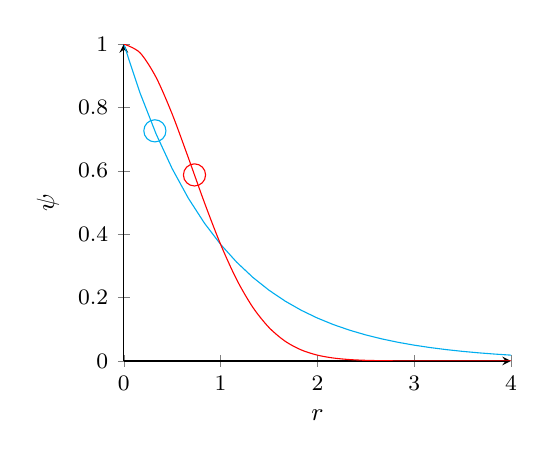
\begin{tikzpicture}[
				remember picture,
			]
			\begin{axis}[
					axis lines=left,
					xlabel=$r$,
					ylabel=$\psi$,
					small,
				]

				\addplot [cyan, domain={0:4}]
				{1*exp(-x)} node [pos=0.1] (n1) {};


				\addplot [red, domain={0:4}, smooth]
				{1*exp(-x^2)} node [pos=0.2] (n2) {};

				%            \fill<1-> [cyan] (n1) circle (2pt);
				%            \fill<2-> [red]  (n2) circle (2pt);

			\end{axis}

			% for debugging purposes only
			\draw [cyan] (n1) circle (4pt);
			\draw [red]  (n2) circle (4pt);
		\end{tikzpicture}
	\end{center}

	\begin{tikzpicture}[
			remember picture,
			overlay,
			arrows={-Latex},
			ultra thick,
		]
		\draw[bend left=45, cyan] (n1) to (pic cs:1);
		\draw[bend right=45,red] (n2) to (pic cs:2);
	\end{tikzpicture}
	%----------------------------------------------------------------------------
\end{frame}
%============================================================================





%============================================================================
\begin{frame}{Недоліки GTO. Контрактація базису}
	%----------------------------------------------------------------------------
	\begin{itemize}
		\item Поведінка GTO не схожа на справжню поведінка АО поблизу ядра, і швидко спадає на нескінченності (на відміну від STO).
		\item Якщо Взяти достатню кількість GTO, можна апроксимувати STO.
	\end{itemize}

	\begin{equation*}
		\tcbhighmath[drop fuzzy shadow]{
			\mathrm{STO} \approx  \sum \mathrm{GTO} ,
		}
	\end{equation*}
	Набір GTO що апроксимують STO --- називається \alert{стисненням}, або \alert{контрактацією} базису.

	\medskip

	{\scriptsize Базиси  STO-NG, де $N$ --- число гаусових функцій (GTO), які \alert{стискують} (\alert{контрактують}) одну орбіталь STO називають \alert{мінімальним базисом}. Під терміном \alert{мінімальний базис} розуміють базисний набір, при якому \alert{число базисних функцій атома визначається числом заповнених оболонок атома}.}
	%    {\small Функції GTO називаються примітивними гаусовими функціями, або примітивами, і таких функцій потрібно істотно більше, ніж STO, але це з лишком компенсується аналітичними виразами для інтегралів.}
	%----------------------------------------------------------------------------
\end{frame}
%============================================================================





%============================================================================
\begin{frame}{Приклад контрактації STO-3G}
	%----------------------------------------------------------------------------
	\begin{equation*}\footnotesize
		\text{STO-3G} =
        {\color{cyan} c_1 \cdot  \left(\frac{2\alpha_1}{\pi}\right)^{3/4}e^{-\alpha_1r^2}
        }
		+
		{\color{magenta!50}
		c_2 \cdot  \left(\frac{2\alpha_2}{\pi}\right)^{3/4}e^{-\alpha_2r^2}
        }
		+
		{\color{green!50!black}
		c_3 \cdot \left(\frac{2\alpha_3}{\pi}\right)^{3/4}e^{-\alpha_3r^2}
        }
	\end{equation*}

	\begin{center}
		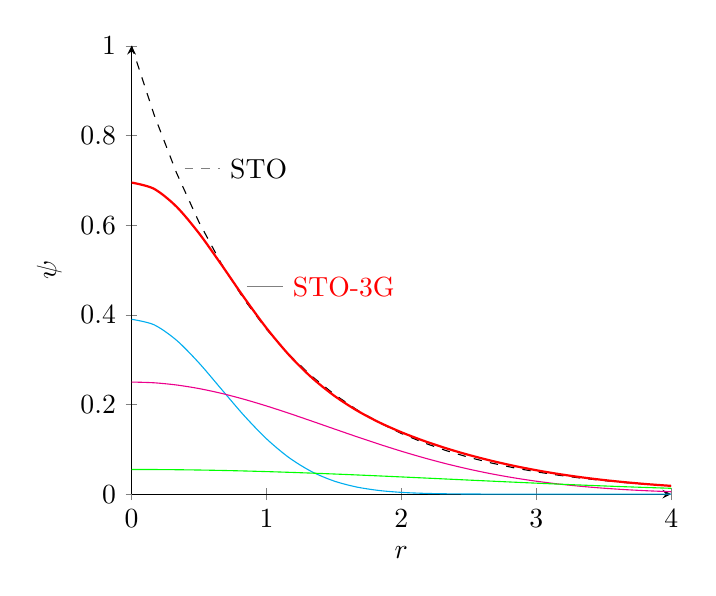
\begin{tikzpicture}[remember picture]
			\begin{axis}[
					axis lines=left,
					xlabel=$r$,
					ylabel=$\psi$,
				]
				\newcommand{\es}{0.39*exp(-1.15*x^2)}
				\newcommand{\p}{0.25*exp(-0.24*x^2)}
				\newcommand{\de}{0.055*exp(-0.09*x^2)}
				\addplot [dashed, domain={0:4}]
				{1*exp(-x)} node [pos=0.1, pin=0:STO] (s1) {};


				\addplot [cyan, domain={0:4}, smooth]
				{\es} node [pos=0.1] (g1) {};

				\addplot [magenta, domain={0:4}, smooth]
				{\p} node [pos=0.2] (g2) {};

				\addplot [green, domain={0:4}, smooth]
				{\de} node [pos=0.2] (g3) {};

				\addplot [thick, domain={0:4}, smooth, red]
				{\es + \p +\de} node [pos=0.2, pin=0:STO-3G] (gs) {};

			\end{axis}
		\end{tikzpicture}
	\end{center}

	\begin{tikzpicture}[
			%remember picture,
			overlay,
			arrows={-Latex},
		]
		%\draw<2>[]     (s1) to (pic cs:ge1);
		% \draw[cyan] (g1) edge (ge1);
		% \draw[magenta]  (g2) edge (ge2);
		% \draw[green]  (g3) edge (ge3);
	\end{tikzpicture}
	%----------------------------------------------------------------------------
\end{frame}
%============================================================================





%============================================================================
\begin{frame}[fragile]{Розрахунок атома He в \texttt{ORCA}}
	%----------------------------------------------------------------------------
	\tikz[remember picture,overlay] \node[opacity=0.3,inner sep=0pt, anchor=north east] at (current page.north east){\includegraphics[width=3cm]{orca_logo}};

	\framesubtitle<1>{inp-файл}
	\begin{onlyenv}<1>
		{\scriptsize\color{blue}\ttfamily
			\begin{verbatim}
! RHF SP

%basis # minimal basis STO-6G
 NewGTO He
 S   6
 1   0.6598456824E+02       0.9163596281E-02
 2   0.1209819836E+02       0.4936149294E-01
 3   0.3384639924E+01       0.1685383049E+00
 4   0.1162715163E+01       0.3705627997E+00
 5   0.4515163224E+00       0.4164915298E+00
 6   0.1859593559E+00       0.1303340841E+00
  end
end

* xyz 0 1
  He        0.00000        0.00000        0.00000
*

%output
    Print[ P_Basis ] 2
    Print[ P_MOs ] 1
end
\end{verbatim}
		}
	\end{onlyenv}
	\framesubtitle<2>{Базис STO-6G}
	\begin{onlyenv}<2>
		\begin{columns}
			\begin{column}{0.5\linewidth}
				\ttfamily\scriptsize\color{blue}
				Group   1 Type He  : 6s contracted to 1s pattern {6} \\[1em]
				\%basis \# minimal basis STO-6G \\
				\ NewGTO He\\
				\ S   6 \hspace*{8ex}\textcolor{red}{$\alpha_i$} \hspace*{14ex}\textcolor{red}{$C_i$}\\
				\ 1   0.6598456824E+02       0.9163596281E-02\\
				\ 2   0.1209819836E+02       0.4936149294E-01\\
				\ 3   0.3384639924E+01       0.1685383049E+00\\
				\ 4   0.1162715163E+01       0.3705627997E+00\\
				\ 5   0.4515163224E+00       0.4164915298E+00\\
				\ 6   0.1859593559E+00       0.1303340841E+00\\
				\ end\\
				end\\
			\end{column}
			\begin{column}{0.5\linewidth}
				\begin{equation*}\label{}
					\psi = c_1 (1s)_\text{CGTO}.
				\end{equation*}
				де
				\begin{multline*}
					(1s)_\text{STO} \approx  (1s)_\text{CGTO} = \\ = \sum_{s = 1}^6 C_i (1s)_\text{GTO} (\alpha_i)
				\end{multline*}
			\end{column}
		\end{columns}

		\bigskip

		\alert{Результатом роботи програми має бути визначення коефіцієнту $c_1$ та розрахунок властивостей атому на його основі.}
	\end{onlyenv}
	\framesubtitle<3-4>{Результат роботи \texttt{ORCA}}
	\begin{onlyenv}<3>

		Атомні орбіталі (MOLECULAR ORBITALS)

		{\footnotesize\color{blue}\ttfamily
				\begin{NiceTabular}{llc}
					    &    & 0          \\
					    &    & -0.89502   \\
					    &    & \ 2.00000  \\
					    &    & \ -------- \\
					0He & 1s & \ 1.000000 \\
					\CodeAfter
					\begin{tikzpicture}[>=stealth, baseline=-2cm]
						\node (1s)  [fit=(1-3)(1-3)] {} ;
						\draw[<-] (1s.north) -- ++(0,0.5) node[above] (phi) {$\psi_{1s}$};
						\node (oe)  [draw=red,fit=(2-3)(2-3)] {} ;
						\draw[<-] (oe.east) -- ++(0.75,0) node[right] {орбітальна енергія};
						\node (pop) [draw=red,fit=(3-3)(3-3)] {} ;
						\draw[<-] (pop.east) -- ++(0.75,0) node[right] {заселеність орбіталі};
						\node (sto) [fit=(5-2)(5-2)] {} ;
						\draw[<-]  (sto.north) -- ++(90:1) node[above] {$\chi_\text{CGTO}$};
						%
						\node (c1) [draw=red,fit=(5-3)(5-3)] {} ;
						\draw[<-] (c1.east) -- ++(0.75,0) node[right] {$c_1$};
					\end{tikzpicture}
				\end{NiceTabular}
			}

		\bigskip

		\begin{alertblock}{}\small
			В даному випадку одна 1s-орбіталь атому гелію представляється лише однією $s$-орбіталлю STO з коефіцієнтом $c_1 = 1$. Фактично, програмі навіть не довелось виконувати багато циклів ітерації (всього один цикл).
		\end{alertblock}
	\end{onlyenv}

	\begin{onlyenv}<4>
		Енергії атома (TOTAL SCF ENERGY)

		\medskip

		{\scriptsize\color{blue}\ttfamily
			\begin{verbatim}
    Total Energy       :           -2.84629209 Eh             -77.45155 eV

    Components:
    Nuclear Repulsion  :            0.00000000 Eh               0.00000 eV
    Electronic Energy  :           -2.84629209 Eh             -77.45155 eV
    One Electron Energy:           -3.90254008 Eh            -106.19351 eV
    Two Electron Energy:            1.05624798 Eh              28.74197 eV

    Virial components:
    Potential Energy   :           -5.70135990 Eh            -155.14189 eV
    Kinetic Energy     :            2.85506780 Eh              77.69034 eV
    Virial Ratio       :            1.99692627
            \end{verbatim}
		}

		{\small Як видно, результати недостатньо точні. Покращити їх можна, вибравши інший базис \url{https://www.basissetexchange.org/}.}

		Приклад: розрахунок атома \ce{He} \href{https://www.youtube.com/watch?v=wGWfPfClFWQ}{\button{Відео}} та \ce{Li} \href{https://www.youtube.com/watch?v=QINMAkm8mXs}{\button{Відео}}
	\end{onlyenv}
	%----------------------------------------------------------------------------
\end{frame}
%============================================================================





%============================================================================
\begin{frame}[fragile]{Уточнення розрахунків}
	\tikz[remember picture,overlay] \node[opacity=0.3,inner sep=0pt, anchor=north east] at (current page.north east){\includegraphics[width=3cm]{orca_logo}};
	\framesubtitle<1>{Вибір базису}
	\framesubtitle<2>{double-zeta базис}
	%----------------------------------------------------------------------------
	\begin{onlyenv}<1>
		\begin{alertblock}{}
			Використання однієї STO (мінімальний базис) в якості орбіталі --- дає нетостатьо точний результат. Кращі результати будуть якщо використати дві і більше STO для моделювання атомної орбіталі.
		\end{alertblock}

		\medskip

		Базис, в якому атомна орбіталь моделюється двома STO називається двічі розчепленими (\alert{double-zeta}):
		\begin{equation*}
			\psi = c_1 \chi(\zeta_1) + c_2 \chi(\zeta_2),
		\end{equation*}
		де кожна STO $\chi$ задаються окремими GTO.
	\end{onlyenv}
	\begin{onlyenv}<2>
		\vspace*{-1cm}
		\begin{columns}[T]
			\begin{column}{0.5\linewidth}\scriptsize\color{blue}
				\begin{center}
					\textcolor{black}{Базис}
				\end{center}
				\begin{verbatim}

%basis
 NewGTO He
 S 3
   1      38.3549367370      0.0401838903
   2       5.7689081479      0.2613913445
   3       1.2399407035      0.7930391578
 S 1
   1       0.2975781595      1.0000000000
  end
end
    \end{verbatim}
			\end{column}
			\begin{column}{0.5\linewidth}\scriptsize\color{blue}
				\begin{center}
					\textcolor{black}{Орбіталі}
				\end{center}
				\begin{verbatim}
                      0         1
                  -0.91413   1.39986
                   2.00000   0.00000
                  --------  --------
  0He  1s         0.592081 -1.149818
  0He  2s         0.513586  1.186959
\end{verbatim}
			\end{column}
		\end{columns}
		\vspace*{-1cm}
		\[
			\psi_{0} = 0.592081 \cdot \sum_{i = 1}^3 C_i GTO(\alpha_i)  + 0.513586 \cdot C_1  GTO(\alpha_1),
		\]
		\begin{alertblock}\scriptsize
			В результатах розрахунку з'являється ще одна орбіталь $\psi_1$ з коефіцієнтами $-1.149818$ та $1.186959$ і орбітальною енергією $1.39986$, яка не заселена електронами і є артефактом вибору базису. Така орбіталь називається \alert{віртуальною} і фізичного трактування при атомних розрахунках не має.
		\end{alertblock}
	\end{onlyenv}
	\begin{onlyenv}<3>\scriptsize\color{blue}
		\begin{verbatim}
----------------
TOTAL SCF ENERGY
----------------

Total Energy       :           -2.85516045 Eh             -77.69287 eV

Components:
Nuclear Repulsion  :            0.00000000 Eh               0.00000 eV
Electronic Energy  :           -2.85516045 Eh             -77.69287 eV
One Electron Energy:           -3.88201183 Eh            -105.63491 eV
Two Electron Energy:            1.02685138 Eh              27.94205 eV

Virial components:
Potential Energy   :           -5.71028066 Eh            -155.38464 eV
Kinetic Energy     :            2.85512021 Eh              77.69177 eV
Virial Ratio       :            2.00001409
\end{verbatim}
	\end{onlyenv}
	%----------------------------------------------------------------------------
\end{frame}
%============================================================================





%============================================================================
\begin{frame}{Чи є життя після Хартрі-Фока?}{Врахування кореляції електронів}\small
	%----------------------------------------------------------------------------
	{\scriptsize \fullcite[Глава V, \S 5]{Yatsimirsij}}

	\bigskip
	\begin{overprint}
		\onslide<1>
		\begin{enumerate}[\faHandORight]
			\item Хвильова функція задана у вигляді детермінанту Слейтера враховує лише один тип у кореляції електронів, який пов'язаний з орієнтацією спінів ({\scriptsize два електрона з однаковими спінами тримаютьсь подалі один від оного, зменшуючи енергію взаємодії між ними}). \item Для електронів з різ\-но\-на\-прям\-ле\-ни\-ми спінами такої кореляції немає, оскільки обмінний інтеграл дорівнює нулю. Тому для парагелію допускається, що рух кожного з електронів відбувається незалежно від іншого.
			\item Якби рух електронів був скорелюваний таким чином, щоб вони рідше підходили близько один до одного, це зменшило б \alert{кулонівське відштовхування} між ними і знизило б енергію.
		\end{enumerate}
		\onslide<2>
		Хіллераас вибрав функцію основного стану парагелію вигляді:
		\begin{equation*}\label{}
			\Psi = \psi_1(r_1)\psi_2(r_2)(1 - ar_{12}),
		\end{equation*}
		де параметр $a$ який можна підібрати варіаційними методами і який враховує кореляцію (при $a = 0$ кореляції нема).

		\medskip

		\hrulefill

		Розрахунок Хіллераас дав: $\zeta = 1.849$, $а = 0.364$. Повна енергія
		при використанні функції дорівнює $-2.891$ а.о.е., тобто відрізняється від експериментальної лише на $0.3$~\%.

		\vspace*{-1ex}
		\hrulefill

		%		\medskip

		%{\scriptsize Корельована функція відображає зменшення ймовірності знаходження електронів на близьких відстанях і збільшує ймовірність перебування одного електрона подалі від іншого. Як наслідок --- знижується енергія системи, бо зменшується міжелектронне відштовхування.}

	\end{overprint}
	%----------------------------------------------------------------------------
\end{frame}
%============================================================================





%============================================================================
\begin{frame}[allowframebreaks]{Література}\scriptsize
	%----------------------------------------------------------------------------
	\printbibliography
	%----------------------------------------------------------------------------
\end{frame}
%============================================================================





\end{document}